\documentclass[12pt,a4paper]{article}

\newcommand{\AppName}{mbsolver}
\input{version.tex}  % written from pyproject.toml by tools/build_docs.sh
\newcommand{\AppAuthors}{Vahid Anari and Toktam Rashidi}
\newcommand{\AppEmail}{vahid.anari8@gmail.com}
\newcommand{\AppURL}{https://github.com/vahid-anari/mbsolver}

\newcommand{\DocName}{\texorpdfstring{Three-Level ($\Lambda$) Model}{Three-Level (Lambda) Model}}
\usepackage{style}

% ── Convenience macros ────────────────────────────────────────────────────────
\newcommand{\T}{T_0}
\newcommand{\mb}{Maxwell--Bloch}
\newcommand{\E}{\mathcal{E}}
\newcommand{\tE}{\tilde{E}}
\newcommand{\tret}{t_{\mathrm{ret}}}

% ══════════════════════════════════════════════════════════════════════════════
\begin{document}

\DocTitlePage{This document derives the dimensionless \mb{} equations of a
  $\Lambda$-type three-level system solved by
  \code{mbsolver.three\_level.solve\_1d}: two dipole-allowed transitions
  $3\rightarrow1$ and $3\rightarrow2$ share the upper level. It starts from
  the three-level Hamiltonian and proceeds through the rotating-wave and
  slowly-varying-envelope approximations to the final dimensionless system,
  its initial conditions and the scales that connect it to physical values.
  The model and its application to the 6.7~GHz methanol flare in
  S255IR-NIRS3 are described in a paper by the authors that is currently
  under review.}

\tableofcontents
\newpage

% ══════════════════════════════════════════════════════════════════════════════
\section{Level Scheme and Hamiltonian}

\begin{figure}[h]
  \centering
  \begin{tikzpicture}[scale=1.1, every node/.style={font=\small}]
    \draw[thick] (0,0) -- (1.6,0) node[right] {$|1\rangle$};
    \draw[thick] (3.4,1.6) -- (5.0,1.6) node[right] {$|2\rangle$};
    \draw[thick] (1.6,4.0) -- (3.4,4.0) node[right] {$|3\rangle$};
    \draw[<->, thick, accent] (0.8,0.05) -- (2.2,3.95)
      node[midway, left=4pt] {$\E_{31}$, $d_{31}$, $\omega_{31}$};
    \draw[<->, thick, accent] (4.2,1.65) -- (2.8,3.95)
      node[midway, right=4pt] {$\E_{32}$, $d_{32}$, $\omega_{32}$};
    \draw[dashed, gray] (1.6,0.05) -- (3.4,1.55)
      node[midway, below right=-1pt] {forbidden};
  \end{tikzpicture}
  \caption{The $\Lambda$-type three-level system. The upper level $|3\rangle$
  is shared by the dipole-allowed transitions $3\rightarrow1$ and
  $3\rightarrow2$; the transition $1\leftrightarrow2$ is dipole forbidden.
  Level spacings are schematic.}
  \label{fig:levels}
\end{figure}

The molecule has three states $|1\rangle$, $|2\rangle$, $|3\rangle$
(Fig.~\ref{fig:levels}). Taking the energy of $|1\rangle$ as zero, the free
Hamiltonian is
\begin{equation}
  \hat{H}_0 = \hbar\omega_2\,|2\rangle\langle 2| + \hbar\omega_3\,|3\rangle\langle 3|,
\end{equation}
so that the transition frequencies are $\omega_{31} = \omega_3$ and
$\omega_{32} = \omega_3 - \omega_2$. With the dipole matrix elements
$d_{ij} = \langle i|\hat{d}|j\rangle$, $d_{ij} = d_{ji}^*$, and
$d_{12} = 0$ for the forbidden transition, the dipole operator along the
field polarization is
\begin{equation}
  \hat{d} = d_{13}\,|1\rangle\langle 3| + d_{23}\,|2\rangle\langle 3| + \mathrm{h.c.},
\end{equation}
and the interaction with the real electric field $\E(z,t)$ is
\begin{equation}
  \hat{H}_{\mathrm{int}} = -\hat{d}\,\E .
\end{equation}
The total Hamiltonian is $\hat{H} = \hat{H}_0 + \hat{H}_{\mathrm{int}}$.

% ══════════════════════════════════════════════════════════════════════════════
\section{Density-Matrix Equations of Motion}

The medium is described by the density matrix $\rho_{ij}$, normalized so
that the populations $n_i = \rho_{ii}$ are fractions of the total number
density $n_0$ of the three-level molecules: the number density in level $i$
is $n_0 n_i$, and initially $n_1^0 + n_2^0 + n_3^0 = 1$. The
Liouville--von Neumann equation $i\hbar\dot{\hat{\rho}} = [\hat{H},\hat{\rho}]$
gives, with $\rho_{ij} = \rho_{ji}^*$,
\begin{align}
  \dot{\rho}_{11} &= -\frac{i}{\hbar}\,\E\,(\rho_{13}d_{31} - \rho_{31}d_{13}), \\
  \dot{\rho}_{22} &= -\frac{i}{\hbar}\,\E\,(\rho_{23}d_{32} - \rho_{32}d_{23}), \\
  \dot{\rho}_{33} &= \frac{i}{\hbar}\,\E\,(\rho_{13}d_{31} - \rho_{31}d_{13})
                   + \frac{i}{\hbar}\,\E\,(\rho_{23}d_{32} - \rho_{32}d_{23}), \\
  \dot{\rho}_{21} &= -i\omega_2\,\rho_{21} - \frac{i}{\hbar}\,\E\,(\rho_{23}d_{31} - \rho_{31}d_{23}), \\
  \dot{\rho}_{31} &= -i\omega_3\,\rho_{31} - \frac{i}{\hbar}\,\E\,d_{31}(\rho_{33} - \rho_{11})
                   + \frac{i}{\hbar}\,\E\,d_{32}\,\rho_{21}, \\
  \dot{\rho}_{32} &= -i(\omega_3 - \omega_2)\,\rho_{32} - \frac{i}{\hbar}\,\E\,d_{32}(\rho_{33} - \rho_{22})
                   + \frac{i}{\hbar}\,\E\,d_{31}\,\rho_{12}.
\end{align}
The coherence $\rho_{21}$ of the forbidden transition is not driven by the
field directly, but it is generated through the two allowed transitions.

% ══════════════════════════════════════════════════════════════════════════════
\section{Maxwell Wave Equation}

For a field propagating along $z$ and polarized perpendicular to it, with
the polarization parallel to the field and no free charges, currents or
magnetization, Maxwell's equations give the one-dimensional wave equation
\begin{equation}
  \pderiv{^2\E}{z^2} - \frac{1}{c^2}\pderiv{^2\E}{t^2}
  = \frac{1}{\epsilon_0 c^2}\pderiv{^2\mathcal{P}}{t^2},
  \label{eq:wave}
\end{equation}
with the macroscopic polarization
\begin{equation}
  \mathcal{P} = n_0\operatorname{Tr}(\hat{d}\hat{\rho})
  = n_0\bigl(\rho_{31}d_{13} + \rho_{32}d_{23} + \mathrm{c.c.}\bigr).
\end{equation}
Only the coherences of the allowed transitions contribute.

% ══════════════════════════════════════════════════════════════════════════════
\section{Slowly Varying Envelope and Rotating-Wave Approximations}

\subsection{Envelope decomposition}

The field is the sum of two carriers, one resonant with each allowed
transition, with slowly varying complex envelopes $E_{31}$ and $E_{32}$:
\begin{equation}
  \E(z,t) = \tfrac{1}{2}\bigl(E_{31}\,e^{-i\varphi_{31}} + E_{32}\,e^{-i\varphi_{32}}\bigr) + \mathrm{c.c.},
  \qquad
  \varphi_{3j} = \omega_{3j}t - k_{3j}z,
  \qquad k_{3j} = \frac{\omega_{3j}}{c}.
\end{equation}
The coherences are written in the same way,
\begin{equation}
  \rho_{31} = \tfrac{1}{2}R_{31}\,e^{-i\varphi_{31}},
  \qquad
  \rho_{32} = \tfrac{1}{2}R_{32}\,e^{-i\varphi_{32}},
  \qquad
  \rho_{21} = \tfrac{1}{2}R_{21}\,e^{-i(\varphi_{31} - \varphi_{32})},
\end{equation}
and all envelopes vary slowly compared with their carriers (SVEA):
\begin{equation}
  \left|\pderiv{E_{3j}}{t}\right| \ll \omega_{3j}|E_{3j}|, \qquad
  \left|\pderiv{E_{3j}}{z}\right| \ll k_{3j}|E_{3j}|,
\end{equation}
and likewise for $R_{3j}$ \cite{GrossHaroche1982,Benedict1996}. In the rotating-wave approximation (RWA) the
terms oscillating at sums of carrier frequencies, and the terms in which a
field drives the transition it is not resonant with, are dropped. The
detunings
\begin{equation}
  \delta\omega_{31} = \omega_{31} - \omega_3, \qquad
  \delta\omega_{32} = \omega_{32} - (\omega_3 - \omega_2), \qquad
  \delta\omega_{21} = \omega_{31} - \omega_{32} - \omega_2
\end{equation}
appear as $i\,\delta\omega_{ij}R_{ij}$ terms; we take exact resonance,
$\delta\omega_{ij} = 0$.

\subsection{Bloch equations for the envelopes}

Substituting the envelopes into the density-matrix equations and keeping
the resonant terms gives
\begin{align}
  \dot{n}_1 &= \tfrac{1}{2}\operatorname{Re}\!\left[\Bigl(-\tfrac{i d_{31}}{\hbar}E_{31}\Bigr)^{\!*} R_{31}\right], \\
  \dot{n}_2 &= \tfrac{1}{2}\operatorname{Re}\!\left[\Bigl(-\tfrac{i d_{32}}{\hbar}E_{32}\Bigr)^{\!*} R_{32}\right], \\
  \dot{n}_3 &= -\tfrac{1}{2}\operatorname{Re}\!\left[\Bigl(-\tfrac{i d_{31}}{\hbar}E_{31}\Bigr)^{\!*} R_{31}
              + \Bigl(-\tfrac{i d_{32}}{\hbar}E_{32}\Bigr)^{\!*} R_{32}\right], \\
  \dot{R}_{21} &= \tfrac{1}{2}\left[\Bigl(-\tfrac{i d_{31}}{\hbar}E_{31}\Bigr) R_{32}^*
              + \Bigl(-\tfrac{i d_{32}}{\hbar}E_{32}\Bigr)^{\!*} R_{31}\right], \\
  \dot{R}_{31} &= \Bigl(-\tfrac{i d_{31}}{\hbar}E_{31}\Bigr)(n_3 - n_1)
              - \tfrac{1}{2}\Bigl(-\tfrac{i d_{32}}{\hbar}E_{32}\Bigr) R_{21}, \\
  \dot{R}_{32} &= \Bigl(-\tfrac{i d_{32}}{\hbar}E_{32}\Bigr)(n_3 - n_2)
              - \tfrac{1}{2}\Bigl(-\tfrac{i d_{31}}{\hbar}E_{31}\Bigr) R_{21}^*.
\end{align}
The combinations $-i d_{3j}E_{3j}/\hbar$ (Rabi frequencies) appear
throughout; they define the dimensionless fields in
Section~\ref{sec:dimless}. Populations are conserved,
$\dot n_1 + \dot n_2 + \dot n_3 = 0$.

\subsection{Field equations}

Substituting the field and the polarization into the wave
equation~(\ref{eq:wave}), the terms at each carrier balance separately.
Dropping second derivatives of the envelopes (SVEA),
\begin{equation}
  \pderiv{E_{3j}}{z} + \frac{1}{c}\pderiv{E_{3j}}{t}
  = i\,\frac{n_0 k_{3j} d_{j3}}{2\epsilon_0}\,R_{3j},
  \qquad j = 1, 2.
\end{equation}

% ══════════════════════════════════════════════════════════════════════════════
\section{Retarded Time and Dimensionless Form}
\label{sec:dimless}

\subsection{Retarded time}

In the frame moving with the fields, $z' = z$ and
$\tret = t - z/c$, the operator $\partial_z + c^{-1}\partial_t$ becomes
$\partial_{z'}$ and the field equations are pure propagation equations,
\begin{equation}
  \pderiv{E_{3j}}{z'} = i\,\frac{n_0 k_{3j} d_{j3}}{2\epsilon_0}\,R_{3j},
\end{equation}
while the Bloch equations keep their form with $t \to \tret$.

\subsection{Scaled variables}

Lengths are scaled by the sample length $L$ and times by $\T$,
\begin{equation}
  \xi = \frac{z'}{L}, \qquad \tau = \frac{\tret}{\T},
  \qquad
  \T = \frac{2\epsilon_0\hbar}{n_0 L k_{32} |d_{32}|^2},
  \label{eq:T0}
\end{equation}
and the fields by their Rabi frequencies,
\begin{equation}
  \boxed{\tE_{3j} = -i\,\frac{\T d_{3j}}{\hbar}\,E_{3j}.}
  \label{eq:Etilde}
\end{equation}
The field equations become
\begin{equation}
  \pderiv{\tE_{31}}{\xi} = \frac{n_0 L |d_{31}|^2 k_{31} \T}{2\epsilon_0\hbar}\,R_{31} = \eta\,R_{31},
  \qquad
  \pderiv{\tE_{32}}{\xi} = \frac{n_0 L |d_{32}|^2 k_{32} \T}{2\epsilon_0\hbar}\,R_{32} = R_{32},
\end{equation}
where $\T$ was chosen to make the coupling of the $3\rightarrow2$ field one,
and the coupling of the $3\rightarrow1$ field is
\begin{equation}
  \boxed{\eta = \left|\frac{d_{31}}{d_{32}}\right|^2 \frac{k_{31}}{k_{32}} = d^2\,\omega,
  \qquad d = \left|\frac{d_{31}}{d_{32}}\right|, \qquad \omega = \frac{k_{31}}{k_{32}}.}
  \label{eq:eta}
\end{equation}
$\eta$ is fixed by the spectroscopy of the two transitions; it is not a
free parameter.

\begin{notebox}
  \textbf{Sign of the field equation.} Here $\partial\tE/\partial\xi = +\eta R$,
  while the two-level model has $\partial A'/\partial z' = -\eta R$. Both use
  the same carrier $e^{i(kz-\omega t)}$ and the same coherence envelope
  (upper--lower element $= \tfrac12 R\,e^{i(kz-\omega t)}$); they differ only
  in the phase of the field scale. The two-level model uses
  $A' = A/A_0$ with $A_0 = -i\hbar/(d\,\T)$, i.e.\ $A' = +i\,d\,\T A/\hbar$,
  while Eq.~(\ref{eq:Etilde}) has $-i$. For the same physical field
  $A' = -\tE$, which flips the sign of every field term: the two-level
  equations $\dot w = A'R$, $\dot R = -A'w$, $\partial_{z'}A' = -\eta R$
  correspond here to $\dot n_{32} = -\tE_{32}R_{32}$,
  $\dot R_{32} = \tE_{32}n_{32}$, $\partial_\xi\tE_{32} = R_{32}$.
  Intensities $|\tE|^2$ are the same in both conventions.
\end{notebox}

\subsection{Relaxation and pumping}

Non-coherent processes are added phenomenologically. The population
differences
\begin{equation}
  n_{31} = n_3 - n_1, \qquad n_{32} = n_3 - n_2
\end{equation}
relax towards their reference values $n_{3j}^0$ with times $T_{3j}^{(1)}$,
and the coherences $R_{ij}$ dephase towards $R_{ij}^0$ with times
$T_{ij}^{(2)}$, $ij = 31, 32, 21$. Positive $n_{3j}$ means inversion on the
$3\rightarrow j$ transition. Pumps $\Lambda_{31}$ and $\Lambda_{32}$ act on
the two population differences. In scaled form,
\begin{equation}
  \tau_{ij}^{(k)} = \frac{T_{ij}^{(k)}}{\T}, \qquad
  \tilde{\Lambda}_{3j} = \T\,\Lambda_{3j}.
\end{equation}

\subsection{Final dimensionless equations}

Combining the Bloch equations for $n_3 - n_1$ and $n_3 - n_2$ and using
Eq.~(\ref{eq:Etilde}):

\begin{resultbox}
\begin{align}
  \pderiv{n_{31}}{\tau} &= -\operatorname{Re}\!\left(\tE_{31}^* R_{31} + \tfrac12\tE_{32}^* R_{32}\right)
     - \frac{n_{31} - n_{31}^0}{\tau_{31}^{(1)}} + \tilde{\Lambda}_{31},
  \label{eq:n31}\\[4pt]
  \pderiv{n_{32}}{\tau} &= -\operatorname{Re}\!\left(\tfrac12\tE_{31}^* R_{31} + \tE_{32}^* R_{32}\right)
     - \frac{n_{32} - n_{32}^0}{\tau_{32}^{(1)}} + \tilde{\Lambda}_{32},
  \label{eq:n32}\\[4pt]
  \pderiv{R_{31}}{\tau} &= \tE_{31}\,n_{31} - \tfrac12\tE_{32}\,R_{21}
     - \frac{R_{31} - R_{31}^0}{\tau_{31}^{(2)}},
  \label{eq:R31}\\[4pt]
  \pderiv{R_{32}}{\tau} &= \tE_{32}\,n_{32} - \tfrac12\tE_{31}\,R_{21}^*
     - \frac{R_{32} - R_{32}^0}{\tau_{32}^{(2)}},
  \label{eq:R32}\\[4pt]
  \pderiv{R_{21}}{\tau} &= \tfrac12\left(\tE_{31}R_{32}^* + \tE_{32}^* R_{31}\right)
     - \frac{R_{21} - R_{21}^0}{\tau_{21}^{(2)}},
  \label{eq:R21}\\[4pt]
  \pderiv{\tE_{31}}{\xi} &= \eta\,R_{31}, \qquad
  \pderiv{\tE_{32}}{\xi} = R_{32}.
  \label{eq:fields}
\end{align}
\end{resultbox}

In the paper the fields are written $\tE_1 \equiv \tE_{31}$ and
$\tE_2 \equiv \tE_{32}$, and the pumps are absorbed into the reference
values $n_{3j}^0$ except for the flare pump of Section~\ref{sec:s255}.

\subsection{Real-variable reduction}
\label{subsec:real}

If the initial coherences $R_{ij}^0$ and the entrance fields $\tE_{3j}(0,\tau)$
are real, the right-hand sides of
Eqs.~(\ref{eq:n31})--(\ref{eq:fields}) are real whenever the variables are,
so all variables stay real. Then $\operatorname{Re}(\tE^* R) = \tE R$,
$R_{21}^* = R_{21}$, and the system becomes

\begin{resultbox}
\begin{align}
  \pderiv{n_{31}}{\tau} &= -\left(\tE_{31} R_{31} + \tfrac12\tE_{32} R_{32}\right)
     - \frac{n_{31} - n_{31}^0}{\tau_{31}^{(1)}} + \tilde{\Lambda}_{31},
  \label{eq:rn31}\\[4pt]
  \pderiv{n_{32}}{\tau} &= -\left(\tfrac12\tE_{31} R_{31} + \tE_{32} R_{32}\right)
     - \frac{n_{32} - n_{32}^0}{\tau_{32}^{(1)}} + \tilde{\Lambda}_{32},\\[4pt]
  \pderiv{R_{31}}{\tau} &= \tE_{31}\,n_{31} - \tfrac12\tE_{32}\,R_{21}
     - \frac{R_{31} - R_{31}^0}{\tau_{31}^{(2)}},\\[4pt]
  \pderiv{R_{32}}{\tau} &= \tE_{32}\,n_{32} - \tfrac12\tE_{31}\,R_{21}
     - \frac{R_{32} - R_{32}^0}{\tau_{32}^{(2)}},\\[4pt]
  \pderiv{R_{21}}{\tau} &= \tfrac12\left(\tE_{31}R_{32} + \tE_{32} R_{31}\right)
     - \frac{R_{21} - R_{21}^0}{\tau_{21}^{(2)}},\\[4pt]
  \pderiv{\tE_{31}}{\xi} &= \eta\,R_{31}, \qquad
  \pderiv{\tE_{32}}{\xi} = R_{32}.
  \label{eq:rfields}
\end{align}
\end{resultbox}

\begin{notebox}
  Equations~(\ref{eq:rn31})--(\ref{eq:rfields}) are the system solved by
  \code{mbsolver.three\_level.solve\_1d}: fourth-order Runge--Kutta in
  $\tau$ at each $\xi$, and an explicit step in $\xi$ for the fields. They
  hold unchanged when the relaxation times depend on time.
\end{notebox}

% ══════════════════════════════════════════════════════════════════════════════
\section{Initial and Boundary Conditions}
\label{sec:ics}

\subsection{Populations}

The initial populations are given by the ratios
\begin{equation}
  r_1 = \frac{n_3^0}{n_1^0}, \qquad r_2 = \frac{n_3^0}{n_2^0},
\end{equation}
which, with $n_1^0 + n_2^0 + n_3^0 = 1$, give
\begin{equation}
  n_1^0 = \frac{r_2}{r_1 + r_2 + r_1 r_2}, \qquad
  n_2^0 = \frac{r_1}{r_1 + r_2 + r_1 r_2}, \qquad
  n_3^0 = \frac{r_1 r_2}{r_1 + r_2 + r_1 r_2},
\end{equation}
and the population differences
\begin{equation}
  n_{31}^0 = \frac{r_2(r_1 - 1)}{r_1 + r_2 + r_1 r_2}, \qquad
  n_{32}^0 = \frac{r_1(r_2 - 1)}{r_1 + r_2 + r_1 r_2}.
  \label{eq:n0}
\end{equation}
The $3\rightarrow j$ transition is inverted when $r_j > 1$. The mixed
configuration of the paper, an inverted $3\rightarrow2$ transition with a
non-inverted $3\rightarrow1$ leakage pathway, is $r_1 < 1 < r_2$. The
reference values $n_{3j}^0$ of the relaxation terms are these initial
values, the same at every $\xi$. All physical initial states lie in the
triangle of Fig.~\ref{fig:ics}.

\begin{figure}[h]
  \centering
  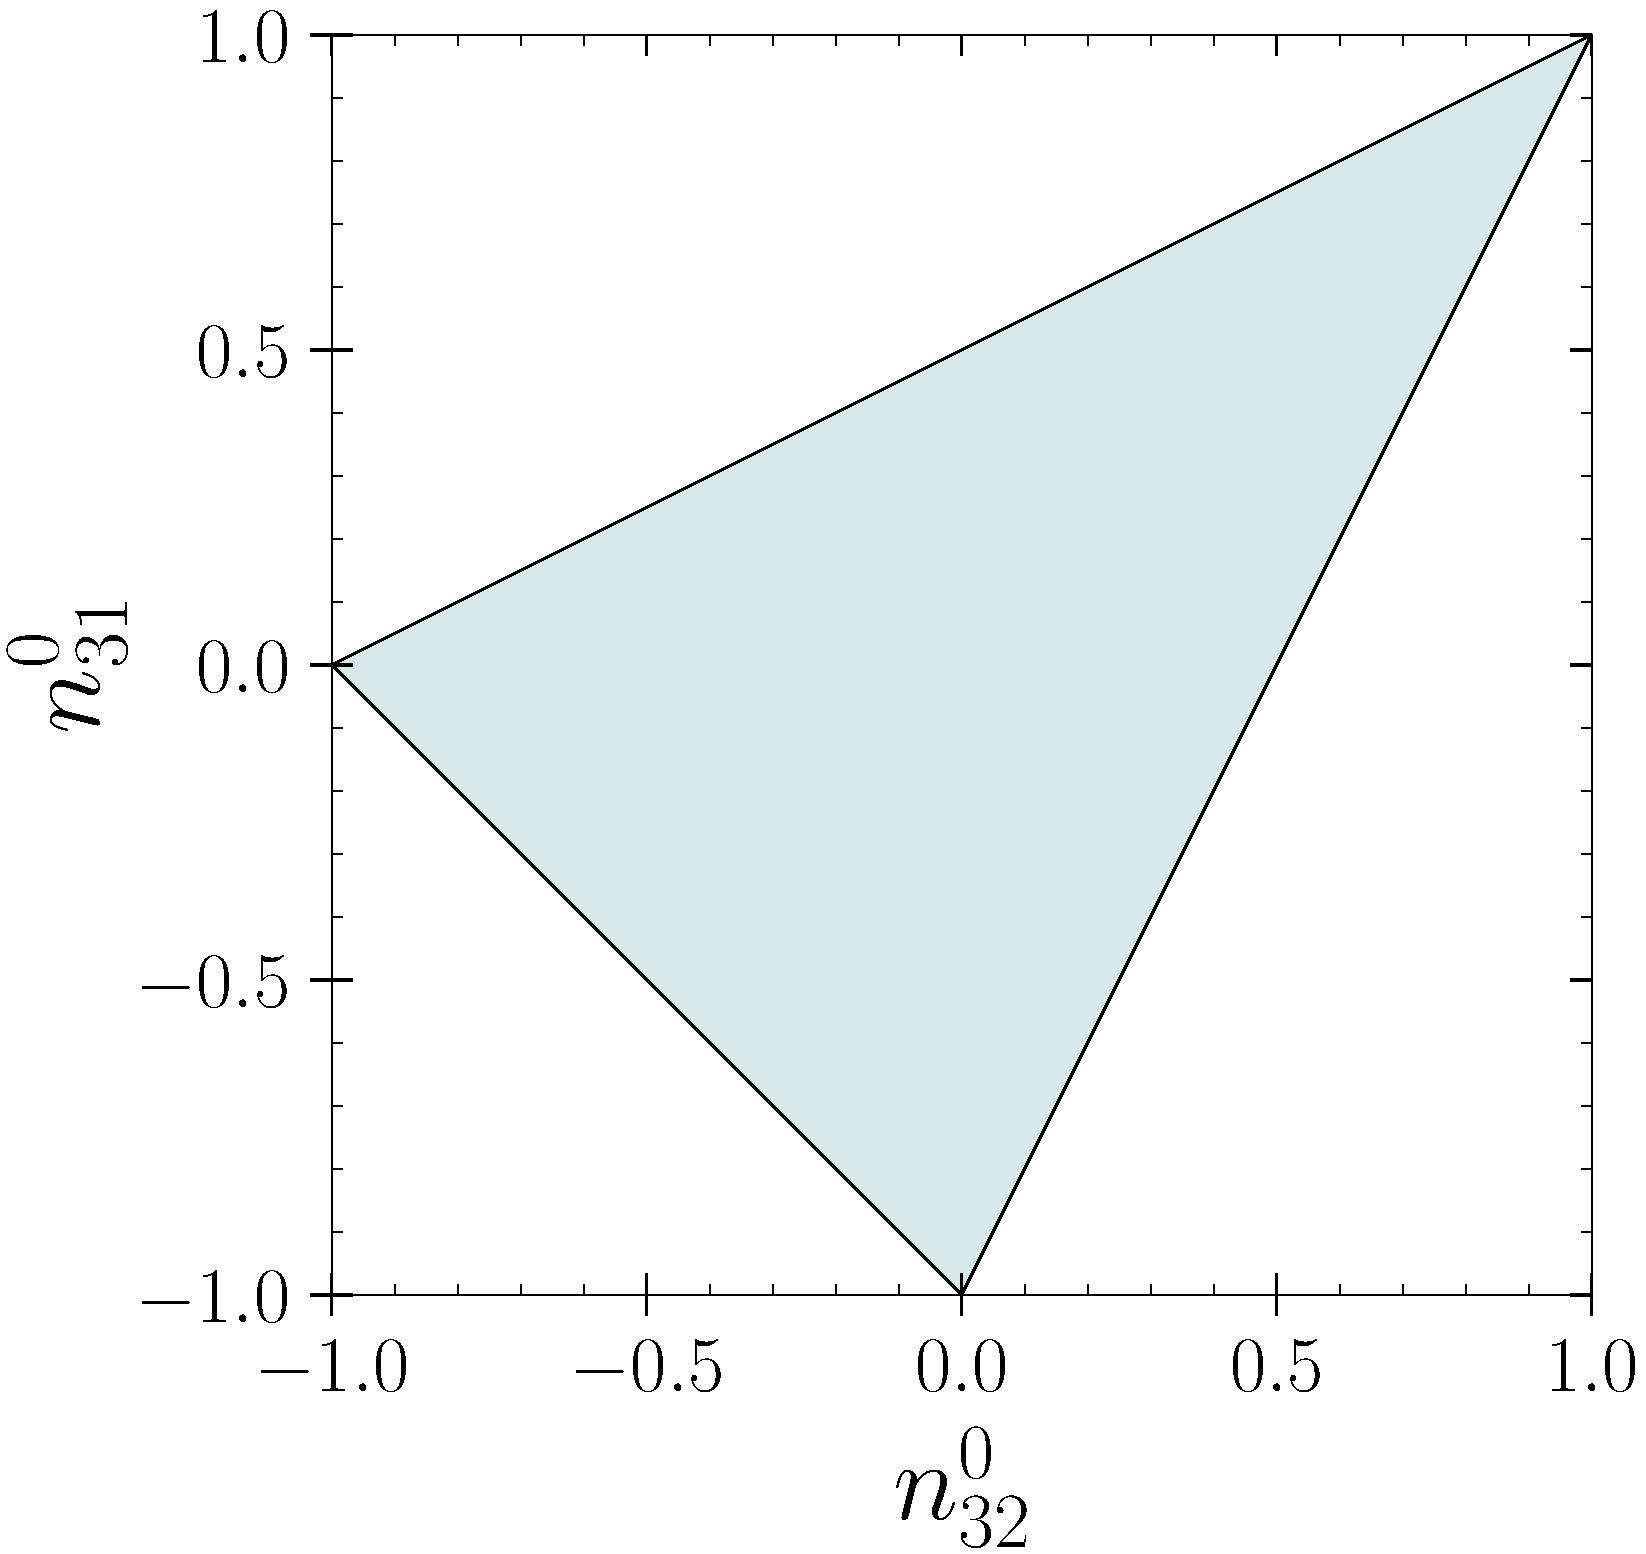
\includegraphics[width=0.45\textwidth]{figures/initial_conditions.pdf}
  \caption{Allowed initial population differences. The corners are all
  molecules in $|3\rangle$ $(1, 1)$, in $|2\rangle$ $(-1, 0)$ and in
  $|1\rangle$ $(0, -1)$.}
  \label{fig:ics}
\end{figure}

\subsection{Coherences}

The magnitude of each initial coherence is bounded by the populations
(Cauchy--Schwarz),
\begin{equation}
  |R_{ij}^0| \le \mathcal{R}_{ij}^{\max} = 2\sqrt{n_i^0 n_j^0},
\end{equation}
and is given as a fraction $c_{ij}$ of this bound,
\begin{equation}
  R_{ij}^0 = c_{ij}\,\mathcal{R}_{ij}^{\max}, \qquad |c_{ij}| \le 1.
\end{equation}
Since no field drives the forbidden transition, the paper takes $c_{21} = 0$.
In terms of $r_1$ and $r_2$,
\begin{equation}
  \mathcal{R}_{31}^{\max} = \frac{2 r_2\sqrt{r_1}}{r_1 + r_2 + r_1 r_2}, \qquad
  \mathcal{R}_{32}^{\max} = \frac{2 r_1\sqrt{r_2}}{r_1 + r_2 + r_1 r_2}, \qquad
  \mathcal{R}_{21}^{\max} = \frac{2\sqrt{r_1 r_2}}{r_1 + r_2 + r_1 r_2}.
\end{equation}

\subsection{Boundary conditions}

The fields entering the sample, $\tE_{3j}(0,\tau)$, are given; for emission
generated by the medium itself they are zero. With uniform initial
coherences, Eq.~(\ref{eq:rfields}) gives the fields at the exit at $\tau = 0$:
$\tE_{31}(1,0) = \tE_{31}(0,0) + \eta R_{31}^0$ and
$\tE_{32}(1,0) = \tE_{32}(0,0) + R_{32}^0$.

% ══════════════════════════════════════════════════════════════════════════════
\section{Physical Scales}
\label{sec:scales}

\subsection{Time scale}

With the Einstein coefficient of the $3\rightarrow2$ transition,
\begin{equation}
  \Gamma_{32} = \frac{\omega_{32}^3 |d_{32}|^2}{3\pi\epsilon_0\hbar c^3}
  = \frac{k_{32}^3 |d_{32}|^2}{3\pi\epsilon_0\hbar},
\end{equation}
the time scale~(\ref{eq:T0}) can be written in the two-level form
\begin{equation}
  \T = \frac{2\epsilon_0\hbar}{n_0 L k_{32} |d_{32}|^2}
     = \frac{2 k_{32}^2}{3\pi\,\Gamma_{32}\, n_0 L}
     = \frac{8\pi}{3\,\Gamma_{32}\, n_0 L \lambda_{32}^2}.
\end{equation}
Both forms agree when $\Gamma_{32}$ is computed from $d_{32}$; with a
measured decay rate they differ by the ratio of the two rates.

\subsection{Fields, intensities and pump}

The dimensionless fields are Rabi frequencies, Eq.~(\ref{eq:Etilde}). In
units of the field scale of the $3\rightarrow2$ transition,
\begin{equation}
  E_0 = \frac{\hbar}{\T |d_{32}|},
\end{equation}
the field amplitudes are $|E_{32}|/E_0 = |\tE_{32}|$ and
$|E_{31}|/E_0 = |\tE_{31}|/d$. Both intensities are therefore given in the
same unit,
\begin{equation}
  I_{31} = I_0\,\frac{|\tE_{31}|^2}{d^2}, \qquad
  I_{32} = I_0\,|\tE_{32}|^2, \qquad
  I_0 = \tfrac12\epsilon_0 c E_0^2,
\end{equation}
and a pump rate $\Lambda$ in $\mathrm{m^{-3}\,s^{-1}}$ (molecules per volume
and time) corresponds to the dimensionless pump
$\tilde{\Lambda} = \Lambda/\Lambda_0$ with $\Lambda_0 = n_0/\T$.

% ══════════════════════════════════════════════════════════════════════════════
\section{In the Code}
\label{sec:code}

\subsection{Solver}

\code{mbsolver.three\_level.solve\_1d} takes the dimensionless parameters
(times in units of $\T$) and returns the variables on \code{n\_planes}
evenly spaced planes $\xi \in [0, 1]$:

\begin{center}
\small
\begin{tabular}{@{}lll@{}}
  \toprule
  Symbol & Argument & Result \\
  \midrule
  $\tau$ grid, $\xi$ grid       & \code{t\_max}, \code{nt}, \code{nz} & \code{res.time}, \code{res.z} \\
  $d$, $\omega$ ($\eta = \omega d^2$) & \code{d}, \code{omega}      & --- \\
  $r_1$, $r_2$                  & \code{r1}, \code{r2}                & --- \\
  $c_{31}$, $c_{32}$, $c_{21}$  & \code{c31}, \code{c32}, \code{c21} (default 0) & --- \\
  $\tau_{31}^{(1)}$, $\tau_{32}^{(1)}$ & \code{t1\_31}, \code{t1\_32} & \code{res.t1\_31}, \code{res.t1\_32} \\
  $\tau_{31}^{(2)}$, $\tau_{32}^{(2)}$, $\tau_{21}^{(2)}$
                                & \code{t2\_31}, \code{t2\_32}, \code{t2\_21} (default $\infty$)
                                & \code{res.t2\_31}, \dots \\
  $\tilde{\Lambda}_{31}$, $\tilde{\Lambda}_{32}$ & \code{pump31}, \code{pump32} & \code{res.pump31}, \code{res.pump32} \\
  $\tE_{31}(0,\tau)$, $\tE_{32}(0,\tau)$ & \code{field31\_in}, \code{field32\_in} & \code{res.field31\_in}, \dots \\
  $\tE_{31}$, $\tE_{32}$        & ---                                 & \code{res.e31}, \code{res.e32} \\
  $|\tE_{31}|^2/d^2$, $|\tE_{32}|^2$ & ---                            & \code{res.intensity31}, \code{res.intensity32} \\
  $n_{31}$, $n_{32}$            & ---                                 & \code{res.n31}, \code{res.n32} \\
  $R_{31}$, $R_{32}$, $R_{21}$  & ---                                 & \code{res.r31}, \code{res.r32}, \code{res.r21} \\
  \bottomrule
\end{tabular}
\end{center}

Relaxation times are numbers or \code{Steps} (\code{math.inf} for none);
pumps and entrance fields are \code{Pulse}s, numbers or lists of them.

\subsection{Helpers}

\code{mbsolver.three\_level.populations(r1, r2)} returns $n_1^0$, $n_2^0$,
$n_3^0$, $n_{31}^0$, $n_{32}^0$ and $\mathcal{R}_{31}^{\max}$,
$\mathcal{R}_{32}^{\max}$, $\mathcal{R}_{21}^{\max}$
(Section~\ref{sec:ics}).

\code{mbsolver.three\_level.scaling(nu31, nu32, d31, d32, l, n0, gamma=None)}
takes the frequencies $\nu_{3j} = \omega_{3j}/2\pi$ (Hz), the dipole moments
(C\,m; \code{mbsolver.constants.DEBYE} converts from debye), $L$ (m) and
$n_0$ (m$^{-3}$) and returns $d$, $\omega$, $\eta$, $k_{3j}$,
$\lambda_{3j}$, $\Gamma_{32}$, $\T$, $E_0$, $I_0$, $10^{26} I_0$
(\code{i0\_jy}, used to plot intensities in Jy) and $\Lambda_0$
(Section~\ref{sec:scales}).
By default $\Gamma_{32}$ is computed from $d_{32}$; \code{gamma} replaces it
with a given rate.

% ══════════════════════════════════════════════════════════════════════════════
\section{Example: S255IR-NIRS3}
\label{sec:s255}

The 6.7~GHz methanol flare in S255IR-NIRS3 was observed with the Toru\'n
32~m telescope \cite{Szymczak2018} during the accretion burst of the
central massive protostar \cite{Caratti2017}. Rajabi et al.\
\cite{Rajabi2019} modelled it as Dicke superradiance \cite{Dicke1954}
with the two-level \mb{} equations used for astrophysical masers
\cite{RajabiHoude2016a,RajabiHoude2016b,RajabiHoude2017}. The three-level
model adds the 239.7~GHz transition, which shares the upper level of the
6.7~GHz line and decays more than four orders of magnitude faster.

\begin{center}
\begin{tabular}{@{}llll@{}}
  \toprule
  Transition & Levels & $\nu$ (MHz) & $d$ (D) \\
  \midrule
  $3\rightarrow1$ & $5_1\,A^+ \rightarrow 4_1\,A^+$ & 239\,746.219 & 0.59425 \\
  $3\rightarrow2$ & $5_1\,A^+ \rightarrow 6_0\,A^+$ & \phantom{00}6\,668.564 & 0.67936 \\
  \bottomrule
\end{tabular}
\end{center}

These give $d = 0.8747$, $\omega = 35.95$ and $\eta = 27.51$. From $d_{3j}$,
$\Gamma_{31} = 5.66\times10^{-5}\ \mathrm{s^{-1}}$ and
$\Gamma_{32} = 1.59\times10^{-9}\ \mathrm{s^{-1}}$.

The sample values are those of the two-level fit: $L = 2.1\times10^{13}$~m,
$\Gamma_{32} = 1.56\times10^{-9}\ \mathrm{s^{-1}}$, initial Bloch angle
$\theta_0 = 4.14\times10^{-10}$ and density $n_0^{(2)} = 1.17\times10^{-6}\
\mathrm{m^{-3}}$ of molecules in levels 2 and 3. The two-level inversion
$\cos\theta_0 = (n_3 - n_2)/(n_3 + n_2)$ fixes
\begin{equation}
  r_2 = \frac{1 + \cos\theta_0}{1 - \cos\theta_0} = \cot^2\frac{\theta_0}{2}
  \simeq 2.33\times10^{19},
\end{equation}
and the three-level density counts level 1 as well,
\begin{equation}
  n_0 = n_0^{(2)}\,\frac{n_1 + n_2 + n_3}{n_2 + n_3}
      = n_0^{(2)}\,\frac{r_1 + r_2 + r_1 r_2}{r_1(1 + r_2)}.
\end{equation}
With $r_1 = 0.94$, $c_{31} = 10^{-10}$ and $c_{32} = 1$, this gives
$n_0 = 2.41\times10^{-6}\ \mathrm{m^{-3}}$ and, with the measured
$\Gamma_{32}$, $\T \simeq 5.24\times10^{4}$~s. The relaxation times
$T_{32}^{(1)} = 1.64\times10^{7}$~s and $T_{32}^{(2)} = 1.55\times10^{6}$~s
are those of the two-level fit, and the $3\rightarrow1$ times are ten times
shorter. The flare is driven by the pump
$\Lambda_{32}(t) = \Lambda_1\,\mathrm{sech}^2[(t - t_p)/T_p]$ with
$\Lambda_1 = 2.6\times10^{-13}\ \mathrm{m^{-3}\,s^{-1}}$ and
$T_p = 8.1\times10^{6}$~s ($\tau_p = T_p/\T \simeq 155$), centred at
$t_p = 795.5\,\T$.

\code{examples/three\_level/s255\_flare.py} runs this case for
$r_1 = 0.79$, 0.89 and 0.94 and plots both intensities in Jy with the
observed 6.7~GHz flux of \cite{Szymczak2018}.

\begin{thebibliography}{99}
\bibitem{Dicke1954}
R.~H. Dicke, Coherence in spontaneous radiation processes,
\emph{Phys.\ Rev.} \textbf{93}, 99 (1954).
\href{https://doi.org/10.1103/PhysRev.93.99}{doi:10.1103/PhysRev.93.99}

\bibitem{GrossHaroche1982}
M.~Gross and S.~Haroche, Superradiance: an essay on the theory of collective
spontaneous emission, \emph{Phys.\ Rep.} \textbf{93}, 301 (1982).
\href{https://doi.org/10.1016/0370-1573(82)90102-8}{doi:10.1016/0370-1573(82)90102-8}

\bibitem{Benedict1996}
M.~G. Benedict, A.~M. Ermolaev, V.~A. Malyshev, I.~V. Sokolov and
E.~D. Trifonov, \emph{Super-radiance: Multiatomic Coherent Emission}
(Institute of Physics Publishing, Bristol, 1996).

\bibitem{RajabiHoude2016a}
F.~Rajabi and M.~Houde, Dicke's superradiance in astrophysics.\ I.\ The
21~cm line, \emph{ApJ} \textbf{826}, 216 (2016).
\href{https://doi.org/10.3847/0004-637X/826/2/216}{doi:10.3847/0004-637X/826/2/216}

\bibitem{RajabiHoude2016b}
F.~Rajabi and M.~Houde, Dicke's superradiance in astrophysics.\ II.\ The
OH 1612~MHz line, \emph{ApJ} \textbf{828}, 57 (2016).

\bibitem{RajabiHoude2017}
F.~Rajabi and M.~Houde, Explaining recurring maser flares in the ISM through
large-scale entangled quantum mechanical states, \emph{Sci.\ Adv.}
\textbf{3}, e1601858 (2017).

\bibitem{Caratti2017}
A.~Caratti o Garatti et al., Disk-mediated accretion burst in a high-mass
young stellar object, \emph{Nat.\ Phys.} \textbf{13}, 276 (2017).
\href{https://doi.org/10.1038/nphys3942}{doi:10.1038/nphys3942}

\bibitem{Szymczak2018}
M.~Szymczak, M.~Olech, P.~Wolak, E.~G\'erard and A.~Bartkiewicz, Giant
burst of methanol maser in S255IR-NIRS3, \emph{A\&A} \textbf{617}, A80
(2018).
\href{https://doi.org/10.1051/0004-6361/201833443}{doi:10.1051/0004-6361/201833443}

\bibitem{Rajabi2019}
F.~Rajabi, M.~Houde, A.~Bartkiewicz, M.~Olech, M.~Szymczak and P.~Wolak,
New evidence for Dicke's superradiance in the 6.7~GHz methanol spectral line
in the interstellar medium, \emph{MNRAS} \textbf{484}, 1590 (2019).
\href{https://doi.org/10.1093/mnras/stz074}{doi:10.1093/mnras/stz074}
\end{thebibliography}

\DocFooter

\end{document}
